%\documentclass[12pt,a4paper]{report}
\documentclass[12pt,a4paper,oneside,onecolumn,openright]{book}
% set the document language
\usepackage[italian]{babel}
% set the encoding used by your editor here (default is utf8)
\usepackage[utf8]{inputenc}
\usepackage[T1]{fontenc}

% math packages
\usepackage{amsmath}
\usepackage{amssymb}
% page margins settings
\usepackage[inner=3cm,outer=2.5cm,top=3cm,bottom=2.5cm]{geometry}
%\usepackage{indentfirst}

% other packages
\usepackage[table]{xcolor}
\usepackage{float}
\usepackage{array}
\usepackage{subfigure}
\usepackage{graphicx}
\usepackage{verbatim}
\usepackage{listings}
\usepackage{url}
\usepackage[hidelinks]{hyperref}
% custom colors
\usepackage{color}
\definecolor{light-gray}{gray}{0.96}
\definecolor{cyan}{RGB}{230,230,255}
\definecolor{dkgreen}{rgb}{0,0.6,0}
\definecolor{gray}{rgb}{0.5,0.5,0.5}
\definecolor{mauve}{rgb}{0.58,0,0.82}

% environment for bash code
\lstset{ %
  language=bash,                % the language of the code
  basicstyle=\footnotesize,           % the size of the fonts that are used for the code
  numbers=left,                   % where to put the line-numbers
  numberstyle=\footnotesize,          % the size of the fonts that are used for the line-numbers
  stepnumber=1,                   % the step between two line-numbers. If it's 1, each line 
                                  % will be numbered
  numbersep=5pt,                  % how far the line-numbers are from the code
  backgroundcolor=\color{white},      % choose the background color. You must add \usepackage{color}
  showspaces=false,               % show spaces adding particular underscores
  showstringspaces=false,         % underline spaces within strings
  showtabs=false,                 % show tabs within strings adding particular underscores
%  frame=single,                   % adds a frame around the code
  rulecolor=\color{black},        % if not set, the frame-color may be changed on line-breaks within not-black text (e.g. commens (green here))
  tabsize=2,                      % sets default tabsize to 2 spaces
  captionpos=b,                   % sets the caption-position to bottom
  breaklines=true,                % sets automatic line breaking
  breakatwhitespace=false,        % sets if automatic breaks should only happen at whitespace
  title=\lstname,                   % show the filename of files included with \lstinputlisting;
                                  % also try caption instead of title
  numberstyle=\tiny\color{gray},        % line number style
  keywordstyle=\textbf,          % keyword style
  commentstyle=\color{dkgreen},       % comment style
%  stringstyle=\color{mauve},         % string literal style
  escapeinside={\%*}{*)},            % if you want to add a comment within your code
  morekeywords={*,...,insert,-}               % if you want to add more keywords to the setù
}

% environment for python code
\lstset{
language=Python,
breaklines=true,
breakatwhitespace=true ,
backgroundcolor=\color{light-gray}
}
% appendices package
%\usepackage{appendix}
% set Appendix name used in the toc
%\renewcommand{\appendixtocname}{Appendice}

% interline
\linespread{1.5}
% set numbers for subsections and show them in the toc
\setcounter{tocdepth}{3} 
\setcounter{secnumdepth}{3}

% layout package, style and settings
\usepackage{fancyhdr}
\pagestyle{fancy}

\fancypagestyle{mainmatter}{%		
		\fancyhf{} 
		\fancyhead{}
		\fancyhead[LE,RO]{\thepage}
		\fancyhead[LO]{\footnotesize{\leftmark}}
		\fancyhead[RE]{\footnotesize{\rightmark}}
		\fancyfoot{}
		\addtolength{\headwidth}{\marginparsep}
		\addtolength{\headheight}{2.5pt}
		\renewcommand{\headrulewidth}{0.3pt}
		\renewcommand{\footrulewidth}{0.0pt}
		}
\fancypagestyle{frontmatter}{%
		\fancyhf{} 
		\fancyhead[LE]{\footnotesize{\MakeUppercase{\thepage}}}
		\fancyhead[RO]{\footnotesize{\MakeUppercase{\thepage}}}
		\fancyhead[RE,LO]{}
		\fancyfoot{}
		\addtolength{\headwidth}{\marginparsep}
		\addtolength{\headheight}{2.5pt}
		\renewcommand{\headrulewidth}{0.0pt}
		\renewcommand{\footrulewidth}{0.0pt}
		}
		
		
\usepackage{fancyhdr}
\pagestyle{fancy}
		\fancyhf{} 
		\fancyhead{}
		\fancyhead[LE,RO]{\thepage} 
		\fancyhead[LO]{\footnotesize{\leftmark}}
		\fancyhead[RE]{\footnotesize{\rightmark}}
		\fancyfoot{}
		\addtolength{\headwidth}{\marginparsep}
		\addtolength{\headheight}{2.5pt}
		\renewcommand{\headrulewidth}{0.3pt}
		\renewcommand{\footrulewidth}{0.0pt}

	\graphicspath{ {images/} }
% empty pages have no numbers
\makeatletter
\def\cleardoublepage{\clearpage\if@twoside \ifodd\c@page\else
\hbox{}
  %Potresti voler togliere il commento dalla linea seguente
  %Questa pagina � stata lasciata intenzionalmente vuota.
\thispagestyle{empty}
\newpage
\if@twocolumn\hbox{}\newpage\fi\fi\fi}
\makeatother
%????
%\textwidth=450pt\oddsidemargin=0pt

%\makeatletter 
%  \DeclareRobustCommand*\textsubscript[1]{% 
%    \@textsubscript{\selectfont#1}} 
%  \newcommand{\@textsubscript}[1]{% 
%    {\m@th\ensuremath{_{\mbox{\fontsize\sf@size\z@#1}}}}} 
\makeatother 

\begin{document}

\begin{titlepage}
\begin{center}
{
    \large
    \textbf{Università  degli studi di Modena e Reggio Emilia} \\
   	\textbf{Dipartimento di Scienze Fisiche, Informatiche e Matematiche} \\
    \vspace{\stretch{0.5}}
    \hspace*{0cm} \hrulefill \hspace*{0cm} \\
    \vspace{\stretch{0.5}}
   	\emph{Corso di Laurea in informatica}
    
	  \vspace{\stretch{12}}
  
  
 		\huge{\bf Titolo: prima riga }}\\
		\vspace{3mm}
		{\huge{\bf Seconda riga}}\\
		\vspace{3mm}
		\vspace{3mm}
		{\huge{\bf Terza riga}}\\
		\vspace{3mm}
		\vspace{3mm}
		{\huge{\bf Quarta riga}}\\
		
		\vspace{\stretch{6}}
		\end{center}
		
\vspace{40mm}
\par
\noindent
\begin{minipage}[t]{0.47\textwidth}
{\large{\bf Relatore:\\
Luca Ferretti}}\\ 
\\

\end{minipage}
\hfill
\begin{minipage}[t]{0.47\textwidth}\raggedleft
{\large{\bf Candidato:\\
Fabio Zanichelli}}
\end{minipage}
\vspace{20mm}
\begin{center}
%\rule[0.1cm]{15.8cm}{0.1mm}
\hspace*{0cm} \hrulefill \hspace*{0cm} \\
{\large{\bf 
Anno Accademico 2021/2022}}
\end{center}

\end{titlepage}

\pagestyle{frontmatter}
\frontmatter

% PAGINA VUOTA
%\clearpage\null\thispagestyle{empty}\clearpage
\setcounter{tocdepth}{2}
\tableofcontents

\setlength{\parindent}{12pt}
\setlength{\parskip}{1ex plus 0.5ex minus 0.2ex}
\mainmatter
\pagestyle{mainmatter}



\chapter{Introduzione}
\label{introduzione}

\section{OS Fingerprinting}
\label{citazioni}

L'OS fingerprinting consiste nel rilevare da remoto il sistema operativo di un dispositivo analizzandone i pacchetti inviati. Le differenze di implementazione dello stack TCP/IP, infatti, determinano comportamenti diversi che, analizzati, consentono di ottenere informazioni utili a questo scopo. \\
Il fingerprinting può essere effettuato in due modalità: attiva e passiva. \\ 
Nella prima si analizzano le risposte ricevute in seguito ad alcuni pacchetti inviati; questi sono appositamente costruiti in modo da massimizzare le informazioni che si possono ottenere dalla risposta.
Nella seconda, invece, viene ispezionato il normale traffico del dispositivo target; si tratta quindi di una tecnica meno invasiva e che si espone meno al rischio di essere scoperti.

\section{Obiettivo}
L'obiettivo consiste nell'analizzare le differenze che portano all'individuazione del sistema operativo, e successivamente modificare determinati parametri di quest'ultimo in modo da riuscire ad ingannare i principali strumenti per il fingereprinting.
I risultati ottenuti, quindi, dovranno essere errati e portare all'individuazione di un sistema operativo differente rispetto a quello realmente in uso.\\
Si è proceduto utilizzando un server HTTP, gestendo quindi pacchetti di non cifrati; si è successivamente cercato di effettuare un'analisi sull'handshake TLS, ovvero sullo scambio di messaggi che precede una comunicazione cifrata.

\section{Strumenti e sistemi operativi utilizzati}
Per la realizzazione dell'obiettivo sono stati utilizzati due differenti sistemi operativi: Windows 11 e Kali (una distribuzione Linux basata su Debian).
La motivazione della scelta di questi sistemi risiede nel fatto che Kali sia stato progettato per la sicurezza informatica, e Windows sia il sistema operativo attualmente più utilizzato; per questa ragione, l'individuazione di quest'ultimo (seppur falsificata) desterebbe meno sospetti. 

I tool utilizzati sono stati i seguenti:
\begin{itemize}
	\item \textbf{Nmap}: principale strumento per effettuare fingerprinting attivo tramite l'invio di specifici pacchetti (\textit{probe}) costruiti appositamente per massimizzare le differenze tra i comportamenti dei sistemi operativi. Consente inoltre di effettuare altre operazioni, alcune delle quali fondamentali per il fingerprinting stesso, come ad esempio il port scanning.
	\item \textbf{p0f}: tool per effettuare fingerprinting passivo. Esso analizza solamente i pacchetti ricevuti da una determinata interfaccia o analizza quelli passati tramite un file con estensione pcap. È anche in grado di effettuare fingerprinting a livello 7.
	\item \textbf{Wireshark}: si tratta di uno strumento che permette la visualizzazione dei pacchetti inviati e ricevuti dal dispositivo tramite un'interfaccia grafica. Consente inoltre di filtrare pacchetti sulla base di determinati campi o protocolli utilizzati.
	\item \textbf{Server Apache}: Web server che consente di rispondere alle richieste di tipo HTTP/HTTPS. È stato installato sia su Windows 11 che su Kali per poter effettuare il confronto tra le risposte inviate.
	\item \textbf{Scapy}: libreria Python in grado di inviare pacchetti modificabili in ogni campo. Molto utile il suo utilizzo per quanto riguarda l'invio di pacchetti "patologici" che stimolano risposte utili ai fini del fingerprinting.
	\item \textbf{nftables}: tool per che permette la modifica o il blocco di pacchetti sulla base del loro contenuto negli header.
\end{itemize}

	







\chapter{Base knowledge}

Per effettuare comunicazioni tramite internet, vi è il bisogno che tutti i dispositivi connessi rispettino determinati meccanismi; questo si rende necessario a causa dell'elevata eterogeneità derivata da hardware e software differenti.
Questi meccanismi, che prendono il nome di \textit{protocolli}, sono strutturati secondo diversi layer (livelli) formando lo stack TCP/IP.  \\
Sebbene l'idea originale (modello ISO/OSI) prevedesse un modello composto da sette livelli, de facto lo schema attualmente in uso ne prevede solamente quattro. Nonostante ciò, nella terminologia informatica la numerazione dei livelli è rimasta quella precedente.
\\
\begin{table}[htb]
	\centering
	\begin{tabular}{| l | c |}
		\hline
		Livello 7 & Applicativo
		\\
		\hline
		Livello 4 & Trasporto
		\\
		\hline
		Livello 3 & Rete
		\\
		\hline
		Livello 2 & Fisico
		\\
		\hline
		
	\end{tabular}
	\caption{Livelli dello stack TCP/IP}
	\label{tab:stack}
\end{table}

\section{Funzionamento dello stack TCP/IP}
Il meccanismo dello stack prevede che ad ogni livello vengano aggiunte al messaggio delle intestazioni (header), a partire dal layer più alto, che verranno valutate dal medesimo livello del ricevente.
Si precisa che l'ordine in cui si valutano gli header dei livelli è inverso rispetto a quello del mittente; il ricevente partirà infatti dal livello più basso.
Questa procedura prende il nome di \textit{incapsulamento} ed è riassunta nella seguente figura:


\begin{figure}[h]
	\centering
	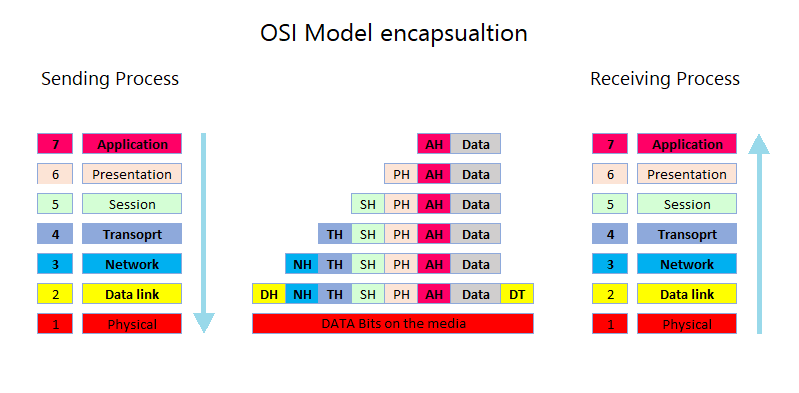
\includegraphics[width=\textwidth]{figures/incapsulamento.png}
	\caption{Incapsulamento nel modello ISO/OSI}
	\label{incapsulamento}
	\cite{incapsulamento}
\end{figure}

\section{Header per il fingerprinting}
Gli header aggiunti ad ogni livello sono formati da vari campi contententi informazioni utili per la comunicazione, e il valore che questi assumono in determinate situazioni è dipendente dal sistema operativo che si sta utilizzando.

Si prenda ad esempio l'header TCP, un protocollo del livello 4 dello stack:\\

\begin{figure}[H]
	\centering
	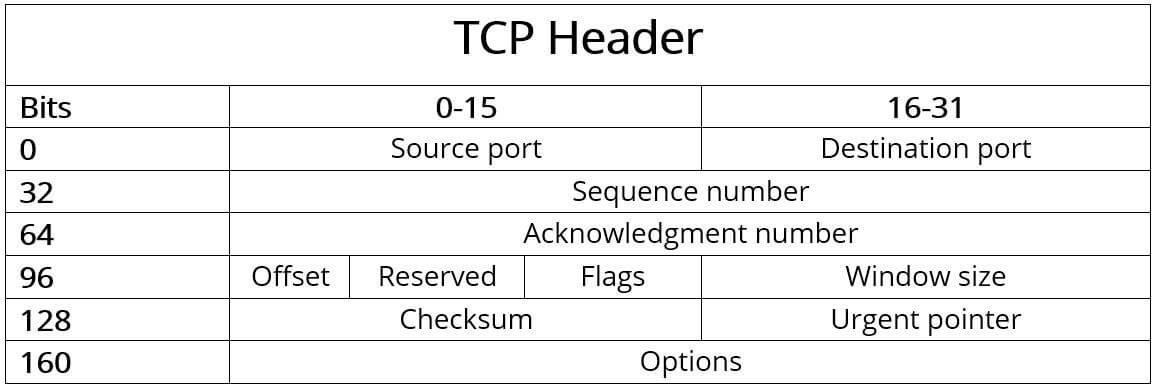
\includegraphics[width=\textwidth]{figures/headerTCP.JPG}
	\caption{Header TCP}
	\label{headerTCP}
	\cite{headerTCP}
\end{figure}

Il campo \textit{option} permette di segnalare al ricevente l'uso di alcune opzioni di comunicazione; il loro supporto e l'effettivo utilizzo, essendo queste facoltative e quindi peculiari di specifici sistemi operativi, rivestono quindi particolare importanza ai fini del fingerprinting.
Esempi analoghi si possono trovare nei protocolli ad ogni livello dello stack, e l'unione delle informazioni acquisite dall'analisi degli header consente di poter individuare con una discreta precisione il sistema operativo del dispositivo target.
\chapter{Analisi}

\section{Procedura}
%L'attività di analisi iniziale, ovvero senza l'ausilio di librerie specifiche per l'invio di determinati pacchetti, è stata effettuata installando un server Apache sia su Windows 11 che su Kali.
%Si è quindi proceduto ad inviare richieste ai server tramite browser web e all'analisi dei pacchetti ricevuti in risposta con l'utilizzo di Wireshark.
%Successivamente sono state analizzate anche le risposte a determinati pacchetti inviati utilizzando la libreria Scapy.
%Di seguito sono riportate le differenze più importanti rilevate durante l'intera attività di analisi.
L'analisi dei pacchetti per l'individuazione delle differenze è stata effettuata sulle risposte ricevute da server Apache installati su Windows 11 e su Kali.
L'attività si analisi è stata svolta in due differenti modalità:
\begin{enumerate}
	\item Nella prima sono state analizzate le risposte ricevute in seguito a richieste GET HTTP inviate tramite browser web; la cattura e l'osservazione di queste è stata effettuata tramite Wireshark.
	\item Nella seconda si è proceduto con l'ispezione delle risposte a specifici pacchetti inviati utilizzando la funzione \textit{sr1} della libreria Python Scapy, che permette la cattura della risposta al pacchetto inviato. Le risposte sono state esaminate con la funzione \textit{show}.
\end{enumerate}
Di seguito vengono mostrate le principali differenze notate tra i due sistemi operativi durante l'intera attività di analisi.

\section{Livello 3: protocolli IP e ICMP}
È stata effettuata in primis l'analisi del TTL (\textit{Time To Live}), essendo un valore estremamente semplice da analizzare.
Questo campo contiene un numero intero positivo che viene decrementato ad ogni \textit{hop}, ovvero ad ogni router che il pacchetto incontra nel percorso verso l'host ricevente, e viene eliminato dalla rete quando questo raggiunge lo 0.
Il protocollo, però, non impone nessun valore di partenza, lasciando libertà di scelta al sistema operativo del mittente; l'unico limite è rappresentato dagli 8 bit riservati a quel campo (ovvero ad un valore massimo di 255).
L'analisi ha portato ad evidenziare la seguente differenza riguardo al TTL:
\begin{table}[H]
	\centering
	\begin{tabular}{| l | c |}
		\hline
		\rowcolor{blue!10} Windows 11 & 128
		\\
		\hline
		\rowcolor{red!10} Kali & 64
		\\
		\hline
		
	\end{tabular}
	\caption{TTL iniziale}
	\label{tab:TTL}
\end{table}

Questa differenza è molto importante in quanto è presente in ogni pacchetto inviato in rete e, se non vengono apportate modifiche, non varia tra un pacchetto e l'altro. Solitamente i valori iniziali sono potenze di due (64 o 128); l'eventuale utilizzo di valori parecchio inusuali denota un comportamento molto riconoscibile.
\\
\\
Inoltre, è stata effettuata l'analisi del protocollo ICMP, e in particolare è stata notata una differenza nel campo \textit{code} in caso di risposta a determinati pacchetti inviati utilizzando la libreria di Python scapy.

\begin{lstlisting}[language=Python, caption={Comando Python per l'invio del pacchetto}]
	from scapy.all import *
	
	pkt = sr1(IP(dst='192.168.63.1')/ICMP(code=9))
	pkt.show()
	
\end{lstlisting}
Questo comando invia un pacchetto ICMP con il campo \textit{code} impostato ad un numero casuale, in questo caso 14: in questo specifico contesto, Windows 11 risponde inviando un pacchetto in cui \textit{code}=0, mentre Kali copia il valore che ha ricevuto nella richiesta.

\begin{table}[h]
	\centering
	\begin{tabular}{ | l | c |}
		\hline
		\rowcolor{blue!10} Windows 11 & 0
		\\
		\hline
		\rowcolor{red!10} Kali & Stesso valore inviato nella richiesta
		\\
		\hline

	\end{tabular}
	\caption{Campo code quando nella richiesta è diverso da 0}
	\label{tab:code}
\end{table}

La differenza è molto peculiare perchè riconoscibile utilizzando solamente il protocollo ICMP (lo stesso del comando \textit{ping}) e non ne influenza il normale utilizzo dal momento che la differenza si presenta solo inviando determinati pacchetti \textit{echo request}.
\section{Livello 4: analisi protocollo TCP}
Il livello 4 dello stack è formato da due protocolli: User Datagram Protocol (UDP) e Transmission Control Protocol (TCP). Entrambi forniscono informazioni utili per il fingerprinting, ma il TCP possiede un numero maggiore di campi e di opzioni utilizzabili, pertanto è stata data priorità all'analisi di quest'ultimo.

Analizzando l'handshake TCP, si può notare una discrepanza nell'utilizzo del Window Scale; quest'opzione consente di aumentare la Window Size oltre il valore che si otterrebbe settando tutti i bit di quel campo a 1.
Ciò è dovuto al fatto che il valore dell'opzione rappresenta il numero di shift verso sinistra dei bit del Window Size, che corrispondono a raddoppi del valore contenuto. 
L'utilizzo di questa opzione viene concordato nei segmenti SYN e SYN+ACK dell'handshake e il suo valore non viene più modificato per il resto della connessione. Confrontando i valori ottenuti da Windows 11 e Kali, si ottiene il seguente risultato:
\\
\begin{table}[htb]
	\centering
	\begin{tabular}{| l | c |}
		\hline
		\rowcolor{blue!10} Windows 11 & 8
		\\
		\hline
		\rowcolor{red!10} Kali & 7
		\\
		\hline
		
	\end{tabular}
	\caption{Window Scaling Factor}
	\label{tab:Window Scale}
\end{table}

Si tratta di una differenza importante, la quale però per essere rilevata necessita del livello 4 dello stack; inoltre, si può osservare solo se si utilizza il protocollo TCP, essendo UDP privo di handshake.
\\
\\
Proseguendo l'analisi si possono notare ulteriori differenze riguardanti il flag sulla notifica esplicita di congestione (ECN). Si tratta di un flag che consente di comunicare a livello end to end una congestione, evitando però la perdita dei pacchetti. Il mittente, infatti, se riceve un pacchetto contenente quest'informazione diminuisce i pacchetti inviati in quella comunicazione, seguendo specifici algoritmi (ad esempio, Reno). 
Se si invia un pacchetto simulando l'inizio di un handshake (SYN) con i flag sulla congestione attivi e si osserva la risposta (SYN+ACK), si possono notare risultati differenti tra i pacchetti ricevuti da Windows 11 e Kali:
\\
\begin{lstlisting}[language=Python, caption={Comando Python per l'invio del pacchetto}]
	from scapy.all import *
	
	pkt=sr1(IP(dst='192.168.63.1')/TCP(dport=80, flags='SCE'))
	pkt.show()
	
\end{lstlisting}

\begin{table}[h]
	\centering
	\begin{tabular}{| l | c |}
		\hline
		\rowcolor{blue!10} Windows 11 & 0
		\\
		\hline
		\rowcolor{red!10} Kali & 1
		\\
		\hline
		
	\end{tabular}
	\caption{ECN in risposta a specifico pacchetto}
	\label{tab:ECN}
\end{table}

Questa diversità è molto importante per il fingerprinting di Nmap che, come verrà meglio specificato nella sezione \ref{algoritmi}, assegna una punteggio elevato al risultato di questo test. 

\section{Livello 7: analisi protocollo HTTP}
Sebbene HTTP sia un protocollo a livello applicativo, esso consente ugualmente di ricavare alcune informazioni utili per l'OS fingerprinting: il campo \textit{User-Agent}, infatti, contiene informazioni esplicite riguardanti il browser che si sta utilizzando e il sistema operativo in utilizzo. Questo tipo di situazione prende il nome di \textit{banner grabbing}.

Inoltre, a questo livello dello stack si può tentare un fingerprinting che vada oltre l'individuazione del sistema operativo, ponendo come obiettivo quello di indovinare il tipo di applicativo in uso.
Questo è reso possibile dal fatto che HTTP è un protocollo di tipo testuale, pertanto non vi sono campi prefissati in determinati bit per ogni funzione.
L'header, infatti, contiene varie coppie secondo lo schema:\\
\textbf{chiave:valore} 


Questo, a differenza dei protocolli analizzati precedentemente, permette un diverso ordine con le quali le coppie vengono elencate, essendo questo ininfluente per una corretta comunicazione; ne consegue che analizzare l'ordinamento è molto importante se si vuole tentare di individuare, ad esempio, il tipo di client in utilizzo.\\

Osservando i pacchetti HTTP inviati dai principali browser web si possono notare delle differenze sull'ordinamento per quanto riguarda Firefox e altri browser basati su Chromium.
L'ordine dei campi nell'header è infatti il seguente:

\begin{table}[h]
	\centering
	\begin{tabular}{| c | c |}
		\hline
		\textbf{Firefox} & \textbf{Chromium-based}
		\\
		\hline
		Host & Host
		\\
		\hline
		User-Agent & Connection
		\\
		\hline
		Accept & Upgrade-Insecure-Requests
		\\
		\hline
		Accept-language & User-Agent
		\\
		\hline
		Accept-Encoding & Accept
		\\
		\hline
		Connection & Accept-Encoding
		\\
		\hline
		Upgrade-Insecure-Requests & Accept-Language
		\\
		\hline
	\end{tabular}
	\caption{Ordine campi header HTTP}
	\label{tab:ordineHTTP}
\end{table}

Inoltre, analizzando i linguaggi accettati si possono osservare ulteriori disuguaglianze riguardanti il campo \textit{Quality Value}.
Si tratta di un valore indicato tramite la lettera q (case insensitive) che esprime la preferenza a determinati linguaggi tramite un numero compreso tra 0 e 1, avente massimo tre cifre decimali; il valore di default è 1 ovvero la massima preferenza \cite{qvalue}. 

Segue la stringa di quello specifico campo riguardante Chrome e Firefox:

\begin{lstlisting} [caption={Campo Accept-Language di Chrome}]
	Acceept-Language: it-IT,it;q=0.9,en-US;q=0.8,en;q=0.7
\end{lstlisting}

\begin{lstlisting}[caption={Campo Accept-Language di Firefox}]
	Acceept-Language: it-IT,it;q=0.8,en-US;q=0.5,en;q=0.3
\end{lstlisting}

Si possono dunque distinguere delle differenze tra i due browser, che ovviamente possono rivestire un ruolo importante in fase di fingerprinting dello User-Agent utilizzato.
\\

È possibile, inoltre, osservare ulteriori differenze che vi sono tra i due browser analizzando il campo \textit{Accept} dell'Header HTTP. Si osservino infatti i due campi nei due browser web menzionati precedentemente:
\\


\begin{lstlisting}[caption={Campo \textit{Accept} di richiesta GET di Chrome}]
	text/html,application/xhtml+xml,application/xml;q=0.9,image/avif,
	image/webp,image/apng,*/*;q=0.8,application/signed-exchange;v=b3;q=0.9
\end{lstlisting}

\begin{lstlisting}[caption={Campo \textit{Accept} di richiesta GET di Firefox}]
	text/html,application/xhtml+xml,application/xml;q=0.9,image/avif,
	image/webp,*/*;q=0.8
\end{lstlisting}


















% PAGINA VUOTA
%\clearpage\null\thispagestyle{empty}\clearpage
%\appendix
%\appendixpage
%\addappheadtotoc

%\clearpage\null\thispagestyle{empty}\clearpage


%\listoffigures


%\begin{flushleft}
%\bibliographystyle{plain}
%\bibliography{sections/references} 
%\end{flushleft}

\end{document}
